
%%%%%%%%%%%%%%%%%%%%%%%%%%%%%%%%%%%%%%%%%%%%%%%%%%%%%%%%%%
% Einstellungen für ganzes Dokument mit Sans-Serif-Schrift
%
%\documentclass[twoside, 
%               a4paper, 
%               10pt, 
%               parskip=full, 
%               sectionentrydots=true, 
%               listof=totoc, 
%               listof=entryprefix, 
%               numbers=endperiod]{scrartcl}
%\renewcommand{\familydefault}{\sfdefault}
%\usepackage[hidelinks]{hyperref}
%\urlstyle{sf}
%\renewcommand\textbullet{\ensuremath{\bullet}}
%
%
%%%%%%%%%%%%%%%%%%%%%%%%%%%%%%%%%%%%%%%%%%%%%%%%%%%%%
% Einstellungen für ganzes Dokument mit Serif-Schrift
%
\documentclass[twoside, 
               a4paper, 
               10pt, 
               parskip=full, 
               sectionentrydots=true, 
               listof=totoc, 
               listof=entryprefix,
               numbers=endperiod]{scrartcl}
\RedeclareSectionCommand[
  beforeskip=0\baselineskip,
  afterskip=.1\baselineskip]{section}
\RedeclareSectionCommand[
  beforeskip=0\baselineskip,
  afterskip=.1\baselineskip]{subsection}
\setkomafont{disposition}{\normalcolor\bfseries}
\usepackage[hidelinks]{hyperref}
%
%
%%%%%%%%%%%%%%%%%%%%%%%%%%%%%%%%%%%%%%%%%%%%%%%%%%%%%

% Einstellen der Seitenränder
\usepackage[top=1.5cm, bottom=2.5cm, left=3cm, right=1.5cm]{geometry}

% Packages für deutsche Umlaute
\usepackage[T1]{fontenc}
\usepackage[ngerman]{babel} 
\usepackage[utf8]{inputenc}

% Packages für und Definiton der "miniSeiten"
\usepackage[most]{tcolorbox}
\newtcolorbox{miniSeite}[1][]{
  enhanced,
  arc=5pt,
  outer arc=5pt,
  colback=white,
  top=10pt,
  bottom=10pt,
  left=20pt,
  right=20pt,
  #1
}

% Package für Seitenlinien (siehe Vorwort)
\usepackage{framed}
\definecolor{isabelline}{rgb}{0.96, 0.94, 0.93}
\renewenvironment{leftbar}[1][\hsize]
{
    \def\FrameCommand
    {
        {\color{gray}\vrule width 3pt}
        \hspace{0pt}
        \fboxsep=\FrameSep\colorbox{isabelline}
    }
    \MakeFramed{\hsize#1\advance\hsize-\width\FrameRestore}
}
{\endMakeFramed}

% Packages für Symbole und Formeln:
\usepackage{amsmath, amssymb, amsthm}

% Theoreme, Sätze, ...
\newtheorem{satz}{Satz}
\newtheorem{theorem}{Theorem}[section]
\newtheorem*{behauptung}{Behauptung}

% Packages für Programm-Listings:
\usepackage{listings}
\usepackage{color}
\definecolor{dkgreen}{rgb}{0,0.6,0}
\definecolor{mauve}{rgb}{0.58,0,0.82}

% Packages um PDF-Dateien einzubinden
\usepackage{pdfpages}

% Packages für Bilder
\usepackage{graphicx}

% Definition eigener Befehle
\newcommand{\frob}{Frobeniushomomorphismus }

% Packages für Stichwortverzeichnis - Standard
\usepackage{makeidx}
\makeindex

% Packages für Stichwortverzeichnis - Formatiert
%\usepackage{imakeidx}
%\usepackage[columns = 1]{idxlayout}
%\makeindex[options= -s my_index_style.ist]
%\usepackage{filecontents}
%\begin{filecontents}{my_index_style.ist}
%headings_flag  1                         % wir benutzen Überschriften
%heading_prefix "{\\bfseries "            % und setzen sie fett
%heading_suffix "\\hfil}\\nopagebreak\n"  % und links, nach innen kein Seitenumbruch
%delim_0 "\\dotfill"                      % Punkte zwischen Einträgen und Seitenzahlen (Ebene 0)
%delim_1 "\\dotfill"                      % Punkte zwischen Einträgen und Seitenzahlen (Ebene 1)
%delim_2 "\\dotfill"                      % Punkte zwischen Einträgen und Seitenzahlen (Ebene 2)
%delim_r "--"                             % Trenner zwischen Start und Ende eines Seitenbereiches
%suffix_2p "\\,f."                        % Suffix bei einem bereich aus 2 Seiten
%suffix_3p "\\,ff."                       % Suffix bei einem bereich aus 3 Seiten
%\end{filecontents}

% Packages für Literaturverzeichnis und Zitierungen
\usepackage[numbers]{natbib}
\bibliographystyle{plainnat}
%\bibliographystyle{humannat}
\renewcommand*{\bibfont}{\raggedright}

% Packages für Tabellen
\usepackage{tabularx}
\usepackage{booktabs}
\newcolumntype{R}[1]{>{\raggedleft\arraybackslash}p{#1}}
\newcolumntype{C}[1]{>{\centering\arraybackslash}p{#1}}

% Package für Abkürzungsverzeichnis mit oder ohne Angabe der Seite
\usepackage[printonlyused]{acronym}
%\usepackage[printonlyused,withpage]{acronym}



\begin{document}

% Erstellen der Titelseite
\begin{center}
  \vspace*{5.5cm}
  \line(1,0){430}\\
  [5mm]
  \Huge \textbf{\LaTeX-Rezepte} \\
  [3mm]
  \line(1,0){430}\\
  \vspace{1.5cm}
  \LARGE\textbf{Problemstellungen und Lösungen}\\
  \vspace{1.5cm}
  \Large\textbf{Peter Kessler}\\  
  \Large\textbf{Januar 2020}\\  
  \vfill
\end{center}
 
\thispagestyle{empty}

% Einfügen einer Leerseite ohne Seitenummer
\newpage
\thispagestyle{empty}
\mbox{}

% Erstellen Vorwort
\newpage
\section*{Vorwort}
\addcontentsline{toc}{section}{Vorwort}

In der Regel werden Texte mit einer Textverarbeitung erstellt. Für professionelle Texte reichen diese aber nicht. So werden an Diplomarbeiten oder Dissertationen höhere Ansprüche gestellt. \LaTeX~ist ein Textsatz-System, das diese Ansprüche erfüllt. Ob in Uni, Fachhochschulen oder höheren Fachschulen - früher oder später stolpern alle über \LaTeX.

Zugegeben: wer an eine Textverarbeitung wie bei OpenOffice, LibreOffice oder Microsoft Office gewohnt ist, wird den Einstieg in \LaTeX~sehr gewöhnungsbedürftig finden. Denn bei \LaTeX~kommt ein umfangreiches Textsatzsystem zum Einsatz, das für Bücher, wissenschaftliche Arbeiten und Artikel gedacht ist.  

\LaTeX~ist ein Softwarepaket, das die Benutzung des Textsatzsystems \TeX~durch die Verwendung von Makros vereinfacht. Das Textsatzsystem wurde einstmals in Hinblick auf die Verschlechterung des Schriftsatzes durch die Einführung von Computern erschaffen und findet heute insbesondere im naturwissenschaftlichen Bereich häufig Anwendung. Gründe dafür sind zum Beispiel die umfangreichen Möglichkeiten, mit denen das System den Satz von mathematischen Symbolen bis hin zu Musiknoten erlaubt. Aber auch im Hinblick auf die notwendigen Formalien wissenschaftlicher Arbeiten hilft \LaTeX~den Autoren dieser Arbeiten dabei, sich hauptsächlich auf den Text zu konzentrieren ohne ihn hierbei mit unnötigen optischen Fragestellungen zu konfrontieren, wie es typischerweise WYSIWYG-Software (z.B. Microsoft Word) tut. Dies allerdings bedeutet auch, dass die Hürden für den Einstieg in \LaTeX~zunächst etwas höher sind als in WYSIWYG-Software, da der unerfahrene Benutzer auf den ersten Blick nicht erkennt, wie sein Dokument letzendlich aussehen wird und wie er Einfluss auf die Gestaltung nehmen kann.

Bei \LaTeX~kümmert man sich nicht fortwährend um das Layout, das man lediglich bei Beginn eines neuen Dokumentes auswählt, sondern in erster Linie um den Text selbst. Früher gab es bei der Textproduktion eine Arbeitsteilung: Der Autor schrieb den Text und ein ausgebildeter Buchsetzer erstellte das Layout. Er kannte sich mit Typographie aus und hatte den Blick für die passende Gestaltung von Schriftgrössen, Zeilenlängen, Fussnoten, Literaturverzeichnissen, Tabellen oder Stichwortlisten. Dies ist wichtig, da ein gutes Layout das Lesen erleichtert und die Verständlichkeit erhöht.

\LaTeX~spielt seinen grossen Vorteil vor allem in Dokumenten mit mathematischen Formeln aus. Denn diese lassen sich mit den entsprechenden \LaTeX-Befehlen direkt in den Text eingeben und werden am Ende automatisch richtig gesetzt. \LaTeX~ist darum im wissenschaftlichen Bereich die erste Wahl für Arbeiten mit Formeln sowie Grafiken und professionellem Layout. 

Wo Licht ist, ist auch immer Schatten. Ein wesentlicher Nachteil soll ebenso Erwähnung finden: 

\begin{leftbar}
Die ersten Schritte mit \LaTeX~sind recht kompliziert, der Einstieg in WYSIWYG-Programme fällt zu Beginn erheblich leichter. Jedoch folgt auf den – zugegeben recht anspruchsvollen – Einstieg ein wesentlich einfacheres Arbeiten als mit erwähnter Konkurrenz.
\end{leftbar}

Die Einarbeitung ist also nicht so einfach wie bei einer normalen Textverarbeitung. Wer bisher nicht programmiert hat, mag beim ersten Blick auf \LaTeX~eingeschüchtert sein, wird dafür aber mit einem Dokument in professionellem Layout belohnt. Zur Erleichterung gibt es zudem hilfreiche Tools.

Das hier vorliegende Dokument enthält eine thematisch geordnete Sammlung verschiedener Problemstellungen und deren Lösung in \LaTeX. Die Beispiele sind so aufgebaut, dass jedes Beispiel ein einziges Thema behandelt. Somit ist gut sichtbar, welche Packages und welche Befehle für die konkrete Problemlösung benötigt werden. 

Grundkenntnisse in \LaTeX~sind für das Verständnis dieses Dokumentes von Vorteil. Haben Sie noch nie mit \LaTeX~gearbeitet, empfehle ich u.a. das Tutorial der TU Graz\footnote{\url{https://latex.tugraz.at/latex/tutorial}}.

Für die ersten praktischen Schritte mit \LaTeX~kann ich Overleaf\footnote{\url{https://de.overleaf.com/}} empfehlen, ein einfach bedienbarer Online-\LaTeX-Editor. Keine Installation notwendig, Versionskontrolle, Hunderte von \LaTeX-Vorlagen und ...
 

% Einfügen einer Leerseite ohne Seitenummer
\newpage
\thispagestyle{empty}
\mbox{}

% Erstellen Inhaltsverzeichnis
\newpage
\tableofcontents \label{toc} 



%%%%%%%%%%%%%%% --- Mathematik --- %%%%%%%%%%%%%%%%%%%

% Linke Seite - Problemstellung Inline Formeln
\newpage
\section{Mathematische Formeln}
\subsection{Inline Formeln}
{\textbf {Ich hätte gerne ...}}

... eine mathematische Formel in meinem Fliesstext.

 
\begin{miniSeite}[colbacktitle=black!35!white,title=Ausdruck]

Pythagoras sagt: Seien $a$ und $b$ die Katheten und $c$ die Hypotenuse, dann gilt: $a^2+b^2=c^2$. Somit gilt für die Hypothenuse: $c=\sqrt{a^2+b^2}$.

\bigskip  
... oder auch ...
\bigskip  

Für $a,b \in \mathbb{R}$ gilt: $(a+b)^{2} = a^{2} + 2ab + b^{2}$

\end{miniSeite}

\LaTeX\ lebt bekanntermassen mit dem Vorurteil, dass es primär für Veröffentlichungen im technisch- resp. naturwissenschaftlichen Bereich entwickelt wurde. Dies ist heutzutage schon lange kein Argument mehr, wenn man auch eindeutig feststellen muss, dass es gerade der Mathematiksatz ist, der \LaTeX\ von anderen Programmen vorteilhaft unterscheidet.


% Rechte Seite - Lösung Inline Formeln
\newpage
{\textbf {Das erreiche ich mit ...}}

... den Packages für die Darstellung mathematischer Formeln und Symbole, die in der Präambel eingebunden werden und indem die Formel im Fliesstext mit je einem \$-Zeichen zu Beginn und am Ende markiert wird.
 
\begin{miniSeite}[colbacktitle=black!35!white,title=\LaTeX-Code]

In der Präambel:

\begin{verbatim}

% für mathematische Symbole und Formeln
\usepackage{amsmath, amssymb}

\end{verbatim}

\tcblower

Im Dokument: 

\begin{verbatim}

Pythagoras sagt: Seien $a$ und $b$ die Katheten und $c$ die Hypotenuse, 
dann gilt: $a^2+b^2=c^2$. Somit gilt für die Hypothenuse: $c=\sqrt{a^2+b^2}$.

\bigskip  
... oder auch ...
\bigskip  

Für $a,b \in \mathbb{R}$ gilt: $(a+b)^{2} = a^{2} + 2ab + b^{2}$

\end{verbatim}

\end{miniSeite}

Der \LaTeX-Befehl \texttt{\char`\\bigskip} wird zwischen die Formel-Sätze und die Zwischenzeile (... oder auch ...) gesetzt um auch in der Textbox (\texttt{tcolorbox}) Abstand zu erhalten. Dieser Befehl hat nichts mit der eigentlichen  Problemstellung zu tun und ist ausserhalb der Textbox nicht notwendig, da der Abstand zwischen den Abschnitten (Paragraphen) in der Dokumentenklasse eingestellt werden kann.

Wie dieses Beispiel zeigt, sind dieser Form Grenzen gesetzt. \LaTeX\ setzt die Formeln so, dass die Zeilenabstände im Fliesstext gleich bleiben. Damit sind dieser Form natürlich Grenzen gesetzt. Brüche, Formeln mit Subscript oder Superscript funktionieren schnell nicht mehr zufriedenstellend. Komplexere Formeln werden besser freigestellt (siehe nächste Beispiele). 




% Linke Seite - Problemstellung Abgesetzte Formeln
\newpage
\subsection{Abgesetzte Formeln}
{\textbf {Ich hätte gerne ...}}

... Formeln die freigestellt (abgesetzt) sind.
 
\begin{miniSeite}[colbacktitle=black!35!white,title=Ausdruck]

Pythagoras sagt: Seien $a$ und $b$ die Katheten und $c$ die
Hypotenuse, dann gilt: 

\begin{displaymath}
  a^2+b^2=c^2 
\end{displaymath}
 
Somit gilt für die Hypothenuse: 

\begin{displaymath}
  c=\sqrt{a^2+b^2} 
\end{displaymath}

\bigskip 
... oder auch ...
\bigskip 
\bigskip 

Für
\begin{displaymath}
a,b \in \mathbb{R}
\end{displaymath}

gilt: 
\begin{displaymath}
\begin{split}
(a+b)^{2} = a^{2} + 2ab + b^{2} \\
(a-b)^{2} = a^{2} - 2ab + b^{2} \\
(a-b)(a+b) = a^{2} - b^{2}
\end{split}
\end{displaymath}

\end{miniSeite}

Zudem sollen die einzelnen Formeln auch auf einer eigenen Zeile ausgedruckt werden.


% Rechte Seite - Lösung Abgesetzte Formeln
\newpage
{\textbf {Das erreiche ich mit ...}}

... den Packages für die Darstellung mathematischer Formeln und Symbole, die in der Präambel eingebunden werden und indem die Formeln in die Mathe-Umgebung \texttt{displaymath} gesetzt werden.
 
\begin{miniSeite}[colbacktitle=black!35!white,title=\LaTeX-Code]

In der Präambel:

\begin{verbatim}

% für mathematische Symbole und Formeln
\usepackage{amsmath, amssymb}

\end{verbatim}

\tcblower

Im Dokument: 

\begin{verbatim}

Pythagoras sagt: Seien $a$ und $b$ die Katheten und $c$ die
Hypotenuse, dann gilt: 

\begin{displaymath}
  a^2+b^2=c^2 
\end{displaymath}
 
Somit gilt für die Hypothenuse: 

\begin{displaymath}
  c=\sqrt{a^2+b^2} 
\end{displaymath}

\bigskip 
... oder auch ...
\bigskip 
\bigskip 

Für
\begin{displaymath}
a,b \in \mathbb{R}
\end{displaymath}

gilt: 
\begin{displaymath}
\begin{split}
(a+b)^{2} = a^{2} + 2ab + b^{2} \\
(a-b)^{2} = a^{2} - 2ab + b^{2} \\
(a-b)(a+b) = a^{2} - b^{2}
\end{split}
\end{displaymath}


\end{verbatim}

\end{miniSeite}

Mit der \LaTeX-Umgebung \texttt{split} können Formeln in der übergeordneten Umgebung \texttt{displaymath} mit \texttt{\char`\\}\texttt{\char`\\} umgebrochen werden.

Der \LaTeX-Befehl \texttt{\char`\\bigskip} wird zwischen die Formel-Sätze und die Zwischenzeile (... oder auch ...) gesetzt um auch in der Textbox (\texttt{tcolorbox}) Abstand zu erhalten. Dieser Befehl hat nichts mit der eigentlichen  Problemstellung zu tun und ist ausserhalb der Textbox nicht notwendig, da der Abstand zwischen den Abschnitten (Paragraphen) in der Dokumentenklasse eingestellt werden kann.

Wie die Formeln am Gleichheitszeichen ausgerichtet werden, wird im nächsten Beispiel gezeigt.




% Linke Seite - Problemstellung abgesetzte, nummerierte und ausgerichtete  Formeln
\newpage
\subsection{Abgesetzte, nummerierte und ausgerichtete Formeln}
{\textbf {Ich hätte gerne ...}}

... Formeln die freigestellt (abgesetzt), ausgerichtet und  nummeriert sind, so dass auf diese im Fliesstext referenziert werden kann.
 
\begin{miniSeite}[colbacktitle=black!35!white,title=Ausdruck]

Da gibt es zwei Formeln, die jedes Kind kennt: 

\begin{align}
  a^2 + b^2 & = c^2     \label{eq:pythagoras}  \\  
  e & = m c^2           \label{eq:einstein}  
\end{align}

Wobei \eqref{eq:pythagoras} Pythagoras und 
\eqref{eq:einstein} Albert Einstein zugeschrieben wird.

\end{miniSeite}

Auch hier sollen die einzelnen Formeln auf einer eigenen Zeile ausgedruckt werden.


% Rechte Seite - Lösung abgesetzte, nummerierte und ausgerichtete  Formeln
\newpage
{\textbf {Das erreiche ich mit ...}}

... den Packages für die Darstellung mathematischer Formeln und Symbole, die in der Präambel eingebunden werden und indem die Formeln in die Mathe-Umgebung \texttt{align} gesetzt werden und die Formeln am Ort des \texttt{\&} Zeichens ausgerichtet werden. 
 
\begin{miniSeite}[colbacktitle=black!35!white,title=\LaTeX-Code]

In der Präambel:

\begin{verbatim}

% für mathematische Symbole und Formeln
\usepackage{amsmath, amssymb}

\end{verbatim}

\tcblower

Im Dokument: 

\begin{verbatim}

Da gibt es zwei Formeln, die jedes Kind kennt: 

\begin{align}
  a^2 + b^2 & = c^2     \label{eq:pythagoras}  \\  
  e & = m c^2           \label{eq:einstein}  
\end{align}

Wobei \eqref{eq:pythagoras} Pythagoras und 
\eqref{eq:einstein} Albert Einstein zugeschrieben wird.

\end{verbatim}

\end{miniSeite}

In der \LaTeX-Umgebung \texttt{align} können Formeln direkt mit \texttt{\char`\\}\texttt{\char`\\} umgebrochen werden.

Um die Formeln referenzieren zu können wird ein Label mit (\texttt{\char`\\label\{<labelname>\}}) gesetzt, auf das im Fliesstext mit \texttt{\char`\\eqref\{<labelname>\}} verwiesen werden kann.

Wie wir hier sehen, wird in der \LaTeX-Umgebung \texttt{align} jede neue Zeile automatisch nummeriert. Wie dies manuell gesteuert resp. unterdrückt werden kann, sehen wir im nächsten Beispiel.




% Linke Seite - Problemstellung abgesetzte, un-/nummerierte und ausgerichtete Formeln
\newpage
\subsection{Abgesetzte, un-/nummerierte und ausgerichtete Formeln}
{\textbf {Ich hätte gerne ...}}

... Formeln die freigestellt (abgesetzt), ausgerichtet und  lediglich die erste der Formeln nummeriert ist, so dass auf diese  im Fliesstext referenziert werden kann.
 
\begin{miniSeite}[colbacktitle=black!35!white,title=Ausdruck]

Da gibt es drei weitere Formeln, die jeder Obenstufenschüler kennt: 

\begin{align}
  (a+b)^{2}  &= a^{2} + 2ab + b^{2}   \label{eq:binome} \\
  (a-b)^{2}  &= a^{2} - 2ab + b^{2}   \nonumber         \\
  (a-b)(a+b) &= a^{2} - b^{2}         \nonumber
\end{align}

Die Binome \eqref{eq:binome}. Binome leiten sich von den Polynomen ab. Polynome sind mathematische Ausdrücke, deren Glieder durch Addition und Subtraktion verbunden sind. Diese Glieder können selber Produkte oder Ähnliches sein. Binome bezeichnen Polynome, die zwei Glieder besitzen. Entsprechend gibt es auch sogenannte Trinome, die drei Glieder besitzen und Monome, die nur aus einem Glied bestehen. 

\bigskip 

Der Binomische Lehrsatz liefert eine Darstellung für beliebig hohe Potenzen eines Binoms:

\begin{equation}
  (a+b)^n = \sum_{k=0}^n \binom{n}{k} a^{n-k} b^k
\end{equation}

\end{miniSeite}

Auch hier sollen die einzelnen Formeln auf einer eigenen Zeile ausgedruckt werden.


% Rechte Seite - Lösung abgesetzte, un-/nummerierte und ausgerichtete Formeln
\newpage
{\textbf {Das erreiche ich mit ...}}

... den Packages für die Darstellung mathematischer Formeln und Symbole, die in der Präambel eingebunden werden und indem die Formeln in die Mathe-Umgebung \texttt{align} gesetzt werden und die Formeln am Ort des \texttt{\&} Zeichens ausgerichtet werden. 
 
\begin{miniSeite}[colbacktitle=black!35!white,title=\LaTeX-Code]

In der Präambel:

\begin{verbatim}

% für mathematische Symbole und Formeln
\usepackage{amsmath, amssymb}

\end{verbatim}

\tcblower

Im Dokument: 

\begin{verbatim}

Da gibt es drei weitere Formeln, die jeder Obenstufenschüler kennt: 

\begin{align}
  (a+b)^{2}  &= a^{2} + 2ab + b^{2}   \label{eq:binome} \\
  (a-b)^{2}  &= a^{2} - 2ab + b^{2}   \nonumber         \\
  (a-b)(a+b) &= a^{2} - b^{2}         \nonumber
\end{align}

Die Binome \eqref{eq:binome}. Binome leiten sich von den Polynomen ab. 
Polynome sind mathematische Ausdrücke, deren Glieder durch Addition und 
Subtraktion verbunden sind. Diese Glieder können selber Produkte oder 
Ähnliches sein. Binome bezeichnen Polynome, die zwei Glieder besitzen. 
Entsprechend gibt es auch sogenannte Trinome, die drei Glieder besitzen 
und Monome, die nur aus einem Glied bestehen. 

\bigskip 

Der Binomische Lehrsatz liefert eine Darstellung für beliebig hohe Potenzen 
eines Binoms:

\begin{equation}
  (a+b)^n = \sum_{k=0}^n \binom{n}{k} a^{n-k} b^k
\end{equation}

\end{verbatim}

\end{miniSeite}

In der \LaTeX-Umgebung \texttt{align} können Formeln direkt mit \texttt{\char`\\}\texttt{\char`\\} umgebrochen werden.

Um die Formeln referenzieren zu können wird ein Label mit (\texttt{\char`\\label\{<labelname>\}}) gesetzt, auf das im Fliesstext mit \texttt{\char`\\eqref\{<labelname>\}} verwiesen werden kann.

Mit \texttt{\char`\\nonumber} oder \texttt{\char`\\notag} kann die Nummerierung manuell unterdrückt werden.




% Linke Seite - Beispiele Formeln
\newpage
\subsection{Beispiele weiterer Formeln}
{\textbf {Folgende Formel(n) ...}}
\begin{miniSeite}[colbacktitle=black!35!white,title=Ausdruck]
\begin{align*}
x&=y           &  w &=z              &  a&=b+c\\
2x&=-y         &  3w&=\frac{1}{2}z   &  a&=b\\
-4 + 5x&=2+y   &  w+2&=-1+w          &  ab&=cb
\end{align*}
\end{miniSeite}
\begin{miniSeite}[colbacktitle=black!35!white,title=Ausdruck]
\begin{displaymath}
\left.
  \begin{cases}
    \multicolumn{1}{@{}c@{\quad}}{\textit{Zeile 1 links}}            \\    
    \multicolumn{1}{@{}c@{\quad}}{\textbf{Zeile 2 links}}            \\
    \multicolumn{1}{@{}c@{\quad}}{\texttt{Zeile 3 links, länger}}    
  \end{cases}
  \mkern-18mu
\right\}
\qquad\longleftarrow\mkern-3mu\longrightarrow\qquad
\left.
  \begin{cases}
    \multicolumn{1}{@{}c@{\quad}}{a^2 + b^2 = c^2}                   \\
    \multicolumn{1}{@{}c@{\quad}}{c = \sqrt[2]{a^2 + b^2}}           \\
    \multicolumn{1}{@{}c@{\quad}}{\text{sagt Pythagoras}}            
  \end{cases}
  \mkern-18mu 
\right\}
\end{displaymath}

\end{miniSeite}

% Rechte Seite - Lösung Beispiele Formeln
\newpage
{\textbf {Wird erstellt mit ...}}
\begin{miniSeite}[colbacktitle=black!35!white,title=\LaTeX-Code]

\begin{verbatim}

\begin{align*}
x&=y           &  w &=z              &  a&=b+c\\
2x&=-y         &  3w&=\frac{1}{2}z   &  a&=b\\
-4 + 5x&=2+y   &  w+2&=-1+w          &  ab&=cb
\end{align*}

\end{verbatim}

\end{miniSeite}
\begin{miniSeite}[colbacktitle=black!35!white,title=\LaTeX-Code]

\begin{verbatim}

\begin{displaymath}
\left.
  \begin{cases}
    \multicolumn{1}{@{}c@{\quad}}{\textit{Zeile 1 links}}            \\    
    \multicolumn{1}{@{}c@{\quad}}{\textbf{Zeile 2 links}}            \\
    \multicolumn{1}{@{}c@{\quad}}{\texttt{Zeile 3 links, länger}}    
  \end{cases}
  \mkern-18mu
\right\}
\qquad\longleftarrow\mkern-3mu\longrightarrow\qquad
\left.
  \begin{cases}
    \multicolumn{1}{@{}c@{\quad}}{a^2 + b^2 = c^2}                   \\
    \multicolumn{1}{@{}c@{\quad}}{c = \sqrt[2]{a^2 + b^2}}           \\
    \multicolumn{1}{@{}c@{\quad}}{\text{sagt Pythagoras}}            
  \end{cases}
  \mkern-18mu 
\right\}
\end{displaymath}


\end{verbatim}

\end{miniSeite}


%%%%%%%%%%%%%%% --- Theorem --- %%%%%%%%%%%%%%%%%%%

% Linke Seite - Problemstellung Theorem Formeln
\newpage
\section{Mathematische Behauptungen und Beweise}
\subsection{Theorem, Proof}

{\textbf {Ich hätte gerne ...}}

... ein Theorem (oder Lemma, oder Proposition, oder Satz, oder Korollar) in meinem Dokument.

Ein Satz oder Theorem ist in der Mathematik eine widerspruchsfreie logische Aussage, die mittels eines Beweises als wahr erkannt, das heisst, aus Axiomen, Definitionen und bereits bekannten Sätzen hergeleitet werden kann.

Ein Satz wird nach seiner Rolle, seiner Bedeutung oder seinem Kontext oft auch anders bezeichnet. Innerhalb eines Artikels oder einer Monografie (z. B. einer Dissertation oder einem Lehrbuch) verwendet man:

\begin{itemize}
\item \textbf{Lemma} (oder Hilfssatz) für eine Aussage, die nur im Beweis anderer Sätze im gleichen Werk verwendet wird und unabhängig davon keine Bedeutung hat,
\item \textbf{Proposition} für eine ebenfalls hauptsächlich lokal bedeutsame Aussage, etwa einen Hilfssatz, der in mehr als einem Beweis verwendet wird,
\item \textbf{Satz} (oder Theorem) für eine wesentliche Erkenntnis, die im Werk dargestellt wird, und
\item \textbf{Korollar} (oder Folgesatz) für eine triviale Folgerung, die sich aus einem Satz oder einer Definition ohne grossen Aufwand ergibt.
\end{itemize}

Die Einordnung eines Satzes in eine der oben genannten Kategorien ist subjektiv und hat keine Folgen für die Verwendung des Satzes. Viele Autoren verzichten auf den Begriff Proposition und setzen dafür Lemma oder Satz ein. Auch Korollar wird nicht immer von Satz unterschieden. Dagegen ist es durchaus üblich und für den Leser hilfreich, wenn reine Hilfssätze als solche erkennbar sind.

Sätze, die allgemein bekannt sind und in der Regel nicht mit der Originalquelle zitiert werden, tragen den Namen des Gegenstandes, über den sie eine Aussage machen oder den Namen des Urhebers oder beides. In diesem Zusammenhang werden auch die Begriffe Fundamentalsatz oder Hauptsatz (eines Gebiets der Mathematik) verwendet, und die Unterscheidung zwischen Satz und Lemma ist oft eher historisch gewachsen als durch Inhalt und Bedeutung bestimmt. Viele Beispiele solcher Namen finden sich in der Liste mathematischer Sätze.
 
\begin{miniSeite}[colbacktitle=black!35!white,title=Ausdruck]

Für Sätze, Lemmata und so weiter stellt LaTeX eine generische Theoremumgebung zur Verfügung. Man kann sich nach seinem Gutdünken Umgebungen zusammenbasteln. Hier einige Beispiele:

\begin{satz} 
   Ein nummerierter Satz. 
\end{satz}

\begin{proof}
   Den wir hier gleich auch mit der Standard-Umgebung proof Beweisen!
\end{proof}

Die Sätze werden automatisch numeriert. Sollen die Sätz in einem Abschnitt die entsprechende Kapitelnummer haben, so sieht das wie folgt aus:

\begin{theorem} 
   Ein nummeriertes Theorem, das die Kapitelnummer enthält. 
\end{theorem}

\begin{proof}
   Das wir hier gleich auch mit der Standard-Umgebung proof Beweisen!
\end{proof}

Theoreme auch ganz ohne Nummer sind möglich:

\begin{behauptung}
   Eine Behauptung
\end{behauptung}

\begin{proof}
   Die wir hier gleich auch mit der Standard-Umgebung proof Beweisen!
\end{proof}

\end{miniSeite}

\textbf{Hinweis:} Für die Erstellung eines Stichwort-/Namensverzeichnis muss ein spezielles \LaTeX-Werkzeug aufgerufen werden (in TeXmaker ist dies MakeIndex - F12). 


% Rechte Seite - Lösung Theorem Formeln
\newpage
{\textbf {Das erreiche ich mit ...}}

... folgender \LaTeX-Befehlssequenz. 
 
\begin{miniSeite}[colbacktitle=black!35!white,title=\LaTeX-Code]

In der Präambel:

\begin{verbatim}

% für mathematische Symbole und Formeln
\usepackage{amsmath, amssymb}

\end{verbatim}

\tcblower

Im Dokument: 

\begin{verbatim}

Da gibt es zwei Formeln, die jedes Kind kennt: 

\begin{align}
  a^2 + b^2 & = c^2     \label{eq:pythagoras}  \\  
  e & = m c^2           \label{eq:einstein}  
\end{align}

Wobei \eqref{eq:pythagoras} Pythagoras und 
\eqref{eq:einstein} Albert Einstein zugeschrieben wird.

\end{verbatim}

\end{miniSeite}

\textbf{Hinweis:} Wie ein Buch in ein Literaturverzeichnis aufgenommen wird und wie ein Literaturverzeichnis erstellt wird, wird in einem sepraten Kapitel (Rezept) gezeigt.




%%%%%%%%%%%%%%% --- Listings --- %%%%%%%%%%%%%%%%%%%

% Linke Seite - Problemstellung Listings 
\newpage
\section{Programm Listings}
\subsection{Matlab, Python, Java, C++}

{\textbf {Ich hätte gerne ...}}

... ein Programm-Listing (Matlab, Python, Java, C++) in meinem Dokument.
 
\begin{miniSeite}[colbacktitle=black!35!white,title=Ausdruck]

Der euklidische Algorithmus ist ein Algorithmus aus dem mathematischen Teilgebiet der Zahlentheorie. Mit ihm lässt sich der grösste gemeinsame Teiler zweier natürlicher Zahlen berechnen. Das Verfahren ist nach dem griechischen Mathematiker Euklid benannt, der es in seinem Werk „Die Elemente“ beschrieben hat.

\bigskip 

Der grösste gemeinsame Teiler zweier Zahlen kann auch aus ihren Primfaktorzerlegungen ermittelt werden. Ist aber von keiner der beiden Zahlen die Primfaktorzerlegung bekannt, so ist der euklidische Algorithmus das schnellste Verfahren zur Berechnung des grössten gemeinsamen Teilers: 

\bigskip 

In Python sieht der euklidische Algorithmus wie folgt aus:

\begin{quote}

\lstinputlisting[language=Python,
    basicstyle=\scriptsize,
    numbers=left,
    numberstyle=\tiny,
    stepnumber=2,
    numbersep=5pt,
    frame=single,
    framerule=0.1pt,
    showstringspaces=false,
    showspaces=false,
    showtabs=false,
    keywordstyle=\color{blue},
    commentstyle=\color{dkgreen},
    stringstyle=\color{mauve},
    backgroundcolor = \color{white}
]{themen/listings/listing_ggT.py}

\end{quote}

\end{miniSeite}

Auch wenn Sie nicht Informatiker sind, möchten Sie in Ihrem Dokument vielleicht Quell-Code zeigen.

\begin{leftbar} 
Dies ist ein weiterer Anwendungsfall, der die Überlegenheit von \LaTeX\ gegenüber WYSIWYG Word Prozessoren aufzeigt. Das Programm-Listing wird aus der Quell-Datei eingelesen und kann mit \LaTeX\ betr. Syntax-Coloring und Syntax-Highlighting der gewohnten Entwicklungsumgebung (IDE) angepasst werden. Damit sehen Programm-Listings im \LaTeX-Dokument aus wie in der gewohnten Entwicklungsumgebung.  
\end{leftbar}

Das Package verfügt über viele weitere Einstellungen zur Darstellung des Quell-Codes. Die Nummerierung der Zeilen ermöglicht zudem, im Fliesstext konkrete Programmzeilen zu referenzieren.


% Rechte Seite - Lösung Listings 
\newpage
{\textbf {Das erreiche ich mit ...}}

... dem Package \texttt{listings} und einigen Einstellungen für Syntax-Coloring und -Highlighting, die in der Präambel eingebunden resp. definiert werden. Die Einstellungen im Dokument für das Listing sind selbsterklärend.
 
\begin{miniSeite}[colbacktitle=black!35!white,title=\LaTeX-Code]

In der Präambel:

\begin{verbatim}

% Packages für Programm-Listings:
\usepackage{listings}
\usepackage{color}
\definecolor{dkgreen}{rgb}{0,0.6,0}
\definecolor{mauve}{rgb}{0.58,0,0.82}

\end{verbatim}

\tcblower

Im Dokument: 

\begin{verbatim}

Der euklidische Algorithmus ist ein Algorithmus aus dem 
mathematischen Teilgebiet der Zahlentheorie. Mit ihm lässt
sich der grösste gemeinsame Teiler zweier natürlicher Zahlen 
berechnen. Das Verfahren ist nach dem griechischen Mathematiker
Euklid benannt, der es in seinem Werk „Die Elemente“ beschrieben hat.

\bigskip 

Der grösste gemeinsame Teiler zweier Zahlen kann auch aus ihren 
Primfaktorzerlegungen ermittelt werden. Ist aber von keiner der 
beiden Zahlen die Primfaktorzerlegung bekannt, so ist der 
euklidische Algorithmus das schnellste Verfahren zur Berechnung 
des grössten gemeinsamen Teilers: 

\bigskip 

In Python sieht der euklidische Algorithmus wie folgt aus:

\begin{quote}

\lstinputlisting[language=Python,
    basicstyle=\scriptsize,
    numbers=left,
    numberstyle=\tiny,
    stepnumber=2,
    numbersep=5pt,
    frame=single,
    framerule=0.1pt,
    showstringspaces=false,
    showspaces=false,
    showtabs=false,
    keywordstyle=\color{blue},
    commentstyle=\color{dkgreen},
    stringstyle=\color{mauve},
    backgroundcolor = \color{white} 
]{themen/listings/listing_ggT.py}

\end{quote}

\end{verbatim}

\end{miniSeite}

Die vielen weiteren Optionen entnehmen Sie bitte der Dokumentation des Package.




%%%%%%%%% --- Fussnoten --- %%%%%%%%%%

% Linke Seite - Problemstellung Fussnoten
\newpage
\section{Fussnoten}
\subsection{Fussnoten setzen}

{\textbf {Ich hätte gerne ...}}

... Fussnoten gesetzt. 
 
\begin{miniSeite}[colbacktitle=black!35!white,title=Ausdruck]

Hier\footnote{Das ist die erste Fussnote} und hier\footnote{Das ist die zweite Fussnote} haben wir zwei unterschiedliche Fussnoten.

\bigskip 
Soll von mehreren Stellen im Dokument auf eine Fussnote\footnote{Das ist eine Fussnote, auf die von mehreren Stellen verwiesen werden soll\label{ftn:multiUse}} verwiesen werden, z.~B. auch von hier\footref{ftn:multiUse} und auch noch von hier\footref{ftn:multiUse}, so muss die entsprechende Fussnote mit einem Label versehen werden und dann wird in den weiteren Malen auf dieses Label verwiesen.

\bigskip
\bigskip 

\end{miniSeite}

\textbf{Hinweis:} Da die Beispiele in diesem Dokument in Textboxes gesetzt sind, sind die Fussnoten hier mit Buchstaben anstelle von Zahlen (\LaTeX\ default). Die Art und Weise wie Fussnoten gesetzt werden, ist genau so wie auf der gegenüberliegenden Seite beschrieben. Sind die Fussnoten nicht in einer Textbox gesetzt, werden diese ganz normal im Dokument durchnummeriert.

\bigskip 
Zur Illustration hier das Gleiche auf einer 'normalen' Seite: 

Hier\footnote{Das ist die erste Fussnote} und hier\footnote{Das ist die zweite Fussnote} haben wir zwei unterschiedliche Fussnoten.

Soll von mehreren Stellen im Dokument auf eine Fussnote\footnote{Das ist eine Fussnote, auf die von mehreren Stellen verwiesen werden soll\label{ftn:multi}} verwiesen werden, z.~B. auch von hier\footref{ftn:multi} und auch noch von hier\footref{ftn:multi}, so muss die entsprechende Fussnote mit einem Label versehen werden und dann wird in den weiteren Malen auf dieses Label verwiesen.


% Rechte Seite - Lösung Fussnoten 
\newpage
{\textbf {Das erreiche ich mit ...}}

... indem ich für die Fussnote auf die mehrfach verwiesen werden soll ein Label setze und dann auf dieses Label verweise.
 
\begin{miniSeite}[colbacktitle=black!35!white,title=\LaTeX-Code]

In der Präambel:

\begin{verbatim}

% keine speziellen Einträge in der Präambel für Fussnoten



\end{verbatim}

\tcblower

Im Dokument: 

\begin{verbatim}



Hier\footnote{Das ist die erste Fussnote} 
und hier\footnote{Das ist die zweite Fussnote} 
haben wir zwei unterschiedliche Fussnoten.

\bigskip 
Soll von mehreren Stellen im Dokument auf eine 
Fussnote\footnote{Das ist eine Fussnote, auf die von 
mehreren Stellen verwiesen werden soll\label{ftn:multiUse}}
verwiesen werden, z.~B. auch von hier\footref{ftn:multiUse} 
und auch noch von hier\footref{ftn:multiUse}, so muss die
entsprechende Fussnote mit einem Label versehen werden und 
dann wird in den weiteren Malen auf dieses Label verwiesen.



\end{verbatim}

\end{miniSeite}

Der \LaTeX-Befehl \texttt{\char`\\bigskip} wird gesetzt um auch in der Textbox Abstand zu erhalten. Dieser Befehl hat nichts mit der eigentlichen  Problemstellung zu tun und ist ausserhalb der Textbox nicht notwendig, da der Abstand zwischen den Abschnitten (Paragraphen) in der Dokumentenklasse eingestellt werden kann.




%%%%%%%%% --- PDF Dateien einbinden --- %%%%%%%%%%

% Linke Seite - Problemstellung PDF Dateien einbinden
\newpage
\section{Einbinden von PDF-Dateien}
\subsection{PDF-Dateien}

{\textbf {Ich hätte gerne ...}}

... eine Vorlage die als PDF-Datei zur Verfügung steht in mein Dokument eingebunden\footnote{\url{https://www.ethz.ch/studierende/de/studium/leistungskontrollen/plagiate.html}}.
 
\begin{miniSeite}[colbacktitle=black!35!white,title=Ausdruck]

Das Einbinden einer ganzen PDF-Vorlagen-Seite kann nicht in einem Minifenster angezeigt werden. Kontrollieren Sie bitte die  Eigenständigkeitserklärung auf Seite \pageref{eigenstaendigkeitserklaerung} in diesem Dokument.

\end{miniSeite}

Beachten Sie bitte nebenstehende Seite.


% Rechte Seite - Lösung PDF Dateien einbinden 
\newpage
{\textbf {Das erreiche ich mit ...}}

... folgender \LaTeX-Befehlssequenz. 
 
\begin{miniSeite}[colbacktitle=black!35!white,title=\LaTeX-Code]

In der Präambel:

\begin{verbatim}

% Packages um PDF-Dateien einzubinden
\usepackage{pdfpages}

\end{verbatim}

\tcblower

Im Dokument (an der Stelle, an der die PDF-Datei eingebunden werden soll): 

\begin{verbatim}

% Einfügen einer Leerseite ohne Seitenummer
\newpage
\thispagestyle{empty}
\mbox{}

% Einbinden der Eigenständigkeitserklärung mit Eintrag in ToC
\newpage
\addcontentsline{toc}{section}{Eigenständigkeitserklärung}
\section*{Eigenständigkeitserklärung
\footnote{Eingebundene PDF-Vorlage der ETH Zürich} 
\label{eigenstaendigkeitserklaerung}}
\begin{figure}
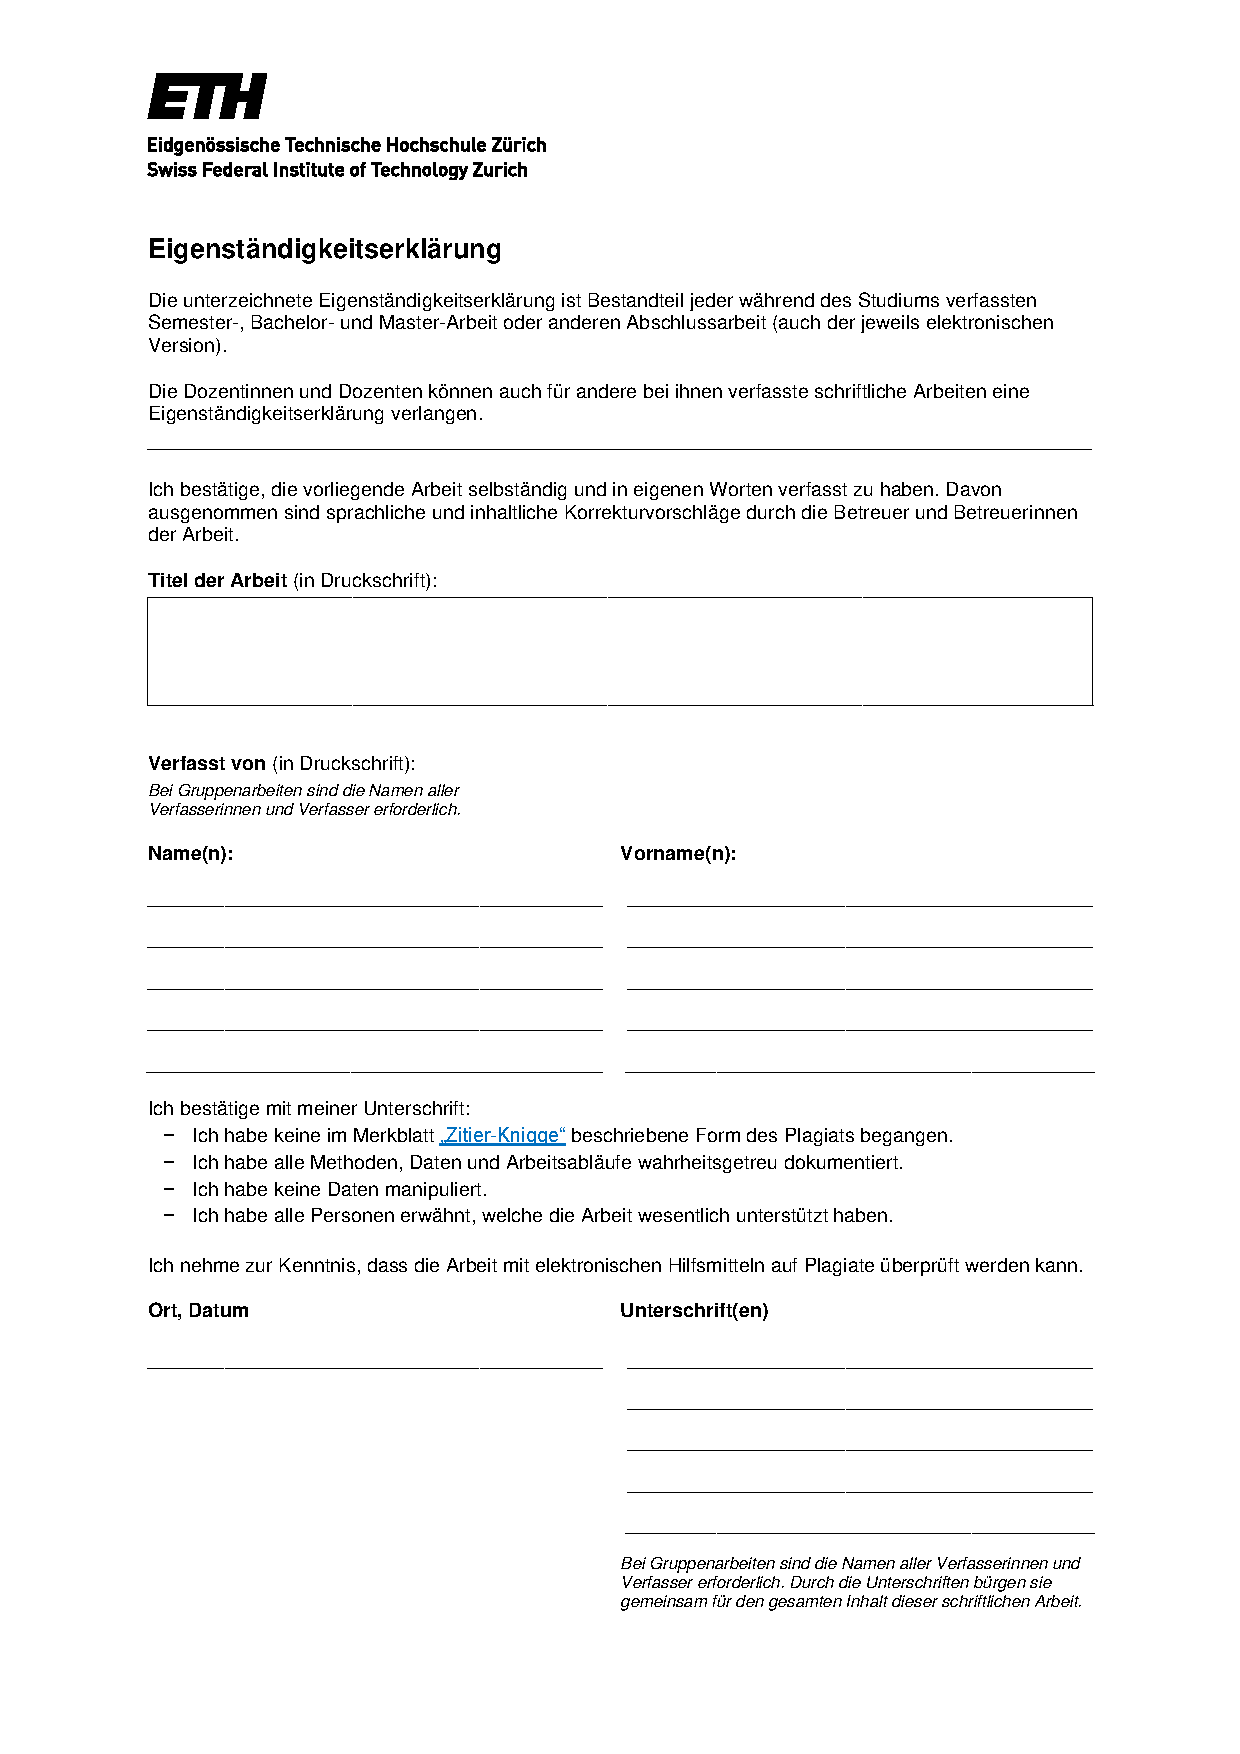
\includepdf[scale=0.8, pagecommand={}]
    {themen/pdfDateien/ethz_eigenstaendigkeitserklaerung.pdf}
\end{figure}

\end{verbatim}

\end{miniSeite}

Die Eigenständigkeitserklärung soll auf einer ungeraden (rechten) Seite des Dokumentes erscheinen.




%%%%%%%%% --- eigene Befehle --- %%%%%%%%%%

% Linke Seite - Problemstellung eigene Befehle
\newpage
\section{Eigene Befehle}
\subsection{Eigene Befehle definieren}

{\textbf {Ich hätte gerne ...}}

... eine einfache Variante um komplizierte, in meiner Arbeit häufig vorkommende Begriffe zu setzen. 
 
\begin{miniSeite}[colbacktitle=black!35!white,title=Ausdruck]

Der \frob ist in der Algebra ein Endomorphismus von Ringen, deren Charakteristik eine Primzahl ist. Der \frob ist nach dem deutschen Mathematiker Ferdinand Georg Frobenius benannt.

\bigskip 
Der Begriff \frob ist schon nicht einfach zu lesen, zu schreiben aber noch einiges mühsamer. 

\bigskip
\bigskip 

\end{miniSeite}

Der Begriff \frob\kern-0.2em\footnote{\url{https://de.wikipedia.org/wiki/Frobeniushomomorphismus}} müsste doch irgendwie einfacher zu setzen sein.

% mit \kern-0.3em wird der Abstand (Leerzeichen) nach 
% dem Begriff zurückgesetzt (Backspace)


% Rechte Seite - Lösung eigene Befehle
\newpage
{\textbf {Das erreiche ich mit ...}}

... der Definition eines eigenen Befehles.
 
\begin{miniSeite}[colbacktitle=black!35!white,title=\LaTeX-Code]

In der Präambel:

\begin{verbatim}

% Definition eigener Befehle
\newcommand{\frob}{Frobeniushomomorphismus }


\end{verbatim}

\tcblower

Im Dokument: 

\begin{verbatim}

Der \frob ist in der Algebra ein Endomorphismus von Ringen, deren
Charakteristik eine Primzahl ist. Der \frob ist nach dem deutschen
Mathematiker Ferdinand Georg Frobenius benannt.

\bigskip 
Der Begriff \frob ist schon nicht einfach zu lesen, zu schreiben
aber noch einiges mühsamer. 

\bigskip
\bigskip 

\end{verbatim}

\end{miniSeite}

Der \LaTeX-Befehl \texttt{\char`\\bigskip} wird gesetzt um auch in der Textbox Abstand zu erhalten. Dieser Befehl hat nichts mit der eigentlichen  Problemstellung zu tun und ist ausserhalb der Textbox nicht notwendig, da der Abstand zwischen den Abschnitten (Paragraphen) in der Dokumentenklasse eingestellt werden kann.




%%%%%%%%% --- Abbildungen & Abbildungsverzeichnis --- %%%%%%%%%%

% Linke Seite - Problemstellung Abbildungen
\newpage
\section{Abbildungen \& Abbildungsverzeichnis}
\subsection{Abbildungen einfügen}

{\textbf {Ich hätte gerne ...}}

... Bilder/Grafiken (inkl. Bildunterschrift für Abbildungsverzeichnis und Label für Referenzierungen im Fliesstext) in mein Dokument eingefügt.
 
%\begin{miniSeite}[colbacktitle=black!35!white,title=Ausdruck]

\vspace{1em}
\hrule
\vspace{1em}

Bilder können mit wenigen Zeilen in \LaTeX eingefügt werden. 

\bigskip 

\bigskip 

\begin{figure}[h!]
\centering
  
\includegraphics[width=0.5\textwidth]{./bilder/LaTeX_Buch.jpg}
  \caption{Wissenschaftliche Arbeiten schreiben mit \LaTeX}
  \label{fig:schlosser}
\end{figure}


\bigskip 

Das Buch in Abbildung \ref{fig:schlosser} auf Seite \pageref{fig:schlosser} ist ein sehr zu empfehlendes Buch zum Thema \LaTeX. 

\vspace{1em}
\hrule
\vspace{1em}

%\end{miniSeite}

\textbf{Hinweis:} Das Einfügen von Bildern in Minifenstern ist sehr umständlich und eher ungewöhnlich. Darum ist das Bild auf dieser Seite nicht in einem Minifenster wie die Beispiele auf den vorhergehenden Seiten.


% Rechte Seite - Lösung Abbildungen 
\newpage
{\textbf {Das erreiche ich mit ...}}

... dem Package für Grafiken, das in der Präambel eingebunden wird und den entsprechenden Befehlen zur Einfügung der Grafik im Dokument.
 
\begin{miniSeite}[colbacktitle=black!35!white,title=\LaTeX-Code]

In der Präambel:

\begin{verbatim}

% Packages für Bilder
\usepackage{graphicx}


\end{verbatim}

\tcblower

Im Dokument: 

\begin{verbatim}

Bilder können mit wenigen Zeilen in \LaTeX eingefügt werden. 

\bigskip 

\begin{figure}[h!]
\centering
  
\includegraphics[width=0.5\textwidth]{./bilder/LaTeX_Buch.jpg}
  \caption{Wissenschaftliche Arbeiten schreiben mit \LaTeX}
  \label{fig:schlosser}
\end{figure}

\bigskip 

Das Buch in Abbildung \ref{fig:schlosser} 
auf Seite \pageref{fig:schlosser} 
ist ein sehr zu empfehlendes Buch zum Thema \LaTeX. 

\end{verbatim}

\end{miniSeite}

\textbf{Hinweis:} Wie ein Buch in ein Literaturverzeichnis aufgenommen wird und wie ein Literaturverzeichnis erstellt wird, wird in einem sepraten Kapitel (Rezept) gezeigt.




% Linke Seite - Problemstellung Abbildungsverzeichnis
\newpage
\subsection{Abbildungsverzeichnis erstellen}
{\textbf {Ich hätte gerne ...}}

... die zuvor eingefügten Abbildungen in einem Abbildungsverzeichnis aufgelistet. Das Abbildungsverzeichnis soll in einem eigenem Kapitel (Section) auf einer eigenen Seite angezeigt werden. Das Kapitel soll nicht nummeriert sein, jedoch trotzdem im Inhaltsverzeichnis angezeigt werden (siehe ToC auf Seite \pageref{toc}).
 
\begin{miniSeite}[colbacktitle=black!35!white,title=Ausdruck]

Das Abbildungsverzeichnis kann nicht in einem Minifenster angezeigt werden. Kontrollieren Sie bitte das Abbildungsverzeichnis auf Seite \pageref{abbildungen} in diesem Dokument.

\end{miniSeite}

Beachten Sie bitte nebenstehende Seite.


% Rechte Seite - Lösung Abbildungsverzeichnis 
\newpage
{\textbf {Das erreiche ich mit ...}}

... folgender \LaTeX-Befehlssequenz. 
 
\begin{miniSeite}[colbacktitle=black!35!white,title=\LaTeX-Code]

In der Präambel:

\begin{verbatim}

% keine weiteren Einträge nötig

\end{verbatim}

\tcblower

Im Dokument (an der Stelle, an der das Stichwortverzeichnis erscheinen soll): 

\begin{verbatim}

% Einfügen einer Leerseite ohne Seitenummer
\newpage
\thispagestyle{empty}
\mbox{}

% Erstellen des Stichwortverzeichisses
% Eintrag in ToC wird automatisch erstellt
\newpage
\label{abbildungen}
\listoffigures


\end{verbatim}

\end{miniSeite}

Das Abbildungsverzeichnis soll auf einer ungeraden (rechten) Seite des Dokumentes erscheinen.




%%%%%%%%% --- Stichworte & Stichwortverzeichnis --- %%%%%%%%%%

% Linke Seite - Problemstellung Stichworte
\newpage
\section{Stichworte \& Stichwortverzeichnis}
\subsection{Stichworte definieren}

{\textbf {Ich hätte gerne ...}}

... Stichworte (Sachworte, Namen) definiert/markiert, damit diese in einem Stichwort-/Namensverzeichnis (Index, Sachwortregister, ...) ausgewiesen werden.
 
\begin{miniSeite}[colbacktitle=black!35!white,title=Ausdruck]

Um einen Begriff (oder Namen) in das Stichwortverzeichnis aufzunehmen, muss dieser entsprechend markiert werden.

\bigskip 

Die Begriffe System\index{System}, Systemzustand\index{System!Zustand} und Systemelement\index{System!Element} sollen im Stichwortverzeichnis aufgenommen werden. 

\bigskip 

Im gedruckten Text ist nicht zu erkennen, ob ein bestimmter Begriff (oder Name) im Stichwortverzeichnis aufgenommen wird.

\end{miniSeite}

\textbf{Hinweis:} Für die Erstellung eines Stichwort-/Namensverzeichnis muss ein spezielles \LaTeX-Werkzeug aufgerufen werden (in TeXmaker ist dies MakeIndex - F12). 


% Rechte Seite - Lösung Stichworte 
\newpage
{\textbf {Das erreiche ich mit ...}}

... dem Package für Stichworte, das in der Präambel eingebunden wird und der entsprechenden Markierung im Fliesstext der Worte, die im Stichwortverzeichnis aufgeführt werden sollen.
 
\begin{miniSeite}[colbacktitle=black!35!white,title=\LaTeX-Code]

In der Präambel:

\begin{verbatim}

% Packages für Stichwortverzeichnis
\usepackage{makeidx}
\makeindex


\end{verbatim}

\tcblower

Im Dokument: 

\begin{verbatim}

Um einen Begriff (oder Namen) in das Stichwortverzeichnis
aufzunehmen, muss dieser entsprechend markiert werden.

\bigskip 

Die Begriffe System\index{System}, Systemzustand\index{System!Zustand} 
und Systemelement\index{System!Element} sollen im Stichwortverzeichnis 
aufgenommen werden. 

\bigskip 

Im gedruckten Text ist nicht zu erkennen, ob ein bestimmter
Begriff (oder Name) im Stichwortverzeichnis aufgenommen wird.

\end{verbatim}

\end{miniSeite}

Somit sind die Stichworte (oder auch Namen) die in das Stichwortverzeichnis aufgenommen werden sollen, markiert/definiert. 




% Linke Seite - Problemstellung Stichwortverzeichnis
\newpage
\subsection{Stichwortverzeichnis erstellen}
{\textbf {Ich hätte gerne ...}}

... die zuvor definierten/markierten Stichworte (Keywords) in einem Stichwortverzeichnis aufgelistet. Das Stichwortverzeichnis soll in einem eigenem Kapitel (Section) auf einer eigenen Seite angezeigt werden. Das Kapitel soll nicht nummeriert sein, jedoch trotzdem im Inhaltsverzeichnis angezeigt werden (siehe Inhaltsverzeichnis auf Seite \pageref{toc}).
 
\begin{miniSeite}[colbacktitle=black!35!white,title=Ausdruck]

Das Stichwortverzeichnis kann nicht in einem Minifenster angezeigt werden. Kontrollieren Sie bitte das Stichwortverzeichnis auf Seite \pageref{index} in diesem Dokument.

\end{miniSeite}

Beachten Sie bitte nebenstehende Seite.


% Rechte Seite - Lösung Stichwortverzeichnis 
\newpage
{\textbf {Das erreiche ich mit ...}}

... folgender \LaTeX-Befehlssequenz. 
 
\begin{miniSeite}[colbacktitle=black!35!white,title=\LaTeX-Code]

In der Präambel:

\begin{verbatim}

% Packages für Stichwortverzeichnis
\usepackage{makeidx}
\makeindex

\end{verbatim}

\tcblower

Im Dokument (an der Stelle, an der das Stichwortverzeichnis erscheinen soll): 

\begin{verbatim}

% Einfügen einer Leerseite ohne Seitenummer
\newpage
\thispagestyle{empty}
\mbox{}

% Erstellen des Stichwortverzeichisses mit Eintrag in ToC
\newpage
\addcontentsline{toc}{section}{Stichwortverzeichnis}
\renewcommand{\indexname}{Stichwortverzeichnis \bigskip}
\printindex


\end{verbatim}

\end{miniSeite}

Das Stichwortverzeichnis soll auf einer ungeraden (rechten) Seite des Dokumentes erscheinen.

\textbf{Zur Erinnerung:} Die Erstellung des Stichwortverzeichnisses erfodert ein spezielles \LaTeX-Werkzeug (MakeIndex). Damit alles korrekt erstellt wird, muss folgende Sequenz eingehalten werden\footnote{Befehle und Funktionstasten wie in TeXmaker verwendet}:

\begin{enumerate}
\setlength\itemsep{-1em}
\item PDFLaTeX (F6)
\item PDFLaTeX (F6)
\item MakeIndex (F12 - nur wenn Stichwortverzeichnis vorhanden)
\item PDFLaTeX (F6)
\item PDFLaTeX (F6)
\item PDF ansehen (F7)
\end{enumerate}

\textbf{Hinweis:} In den meisten IDEs kann obige Befehls-Sequenz eingestellt werden und über "'schnelles Übersetzen"' mit einem Mausklick ausgeführt werden.




%%%%%%%%% --- Zitieren & Literatur- / Quellenverzeichnis --- %%%%%%%%%%

% Linke Seite - Problemstellung Zitieren
\newpage
\section{Quellen \& Literaturverzeichnis}
\subsection{{Quellen \& Literatur zitieren}}

{\textbf {Ich hätte gerne ...}}

... fremde Quellen und Literatur (inkl. Erstellung eines Literaturverzeichnis) zitiert.
 
%\begin{miniSeite}[colbacktitle=black!35!white,title=Ausdruck]
\vspace{1em}
\hrule
\vspace{1em}

\begin{figure}[h!]
\centering
  
\includegraphics[width=0.5\textwidth]{./bilder/LaTeX_Buch.jpg}
  \caption{Eine Buchempfehlung zu \LaTeX}
\end{figure}

\bigskip 

Oben abgebildetes Buch\cite{Schlosser2017} ist ein sehr zu empfehlendes Buch zum Thema \LaTeX. 

\vspace{1em}
\hrule
\vspace{1em}

%\end{miniSeite}

\textbf{Hinweis:} Das Einfügen von Bildern in Minifenstern ist sehr umständlich und eher ungewöhnlich. Darum ist das Bild auf dieser Seite nicht in einem Minifenster wie andere Beispiele auf vorhergehenden Seiten.


% Rechte Seite - Lösung Zitieren 
\newpage
{\textbf {Das erreiche ich mit ...}}

... dem Package für Grafiken, das in der Präambel eingebunden wird und den entsprechenden Befehlen zur Einfügung der Grafik im Dokument.
 
\begin{miniSeite}[colbacktitle=black!35!white,title=\LaTeX-Code]

In der Präambel:

\begin{verbatim}

% Packages für Literaturverzeichnis und Zitierungen
\usepackage[numbers]{natbib}
\bibliographystyle{plainnat}
\renewcommand*{\bibfont}{\raggedright}

\end{verbatim}

\tcblower

Im Dokument: 

\begin{verbatim}

Oben abgebildetes Buch\cite{Schlosser2017} ist ein sehr 
zu empfehlendes Buch zum Thema \LaTeX. 

\end{verbatim}

\end{miniSeite}

Die zitierten Quellen müssen in einer bib-Datei erfasst sein, anhand derer \LaTeX\ dann ein Literaturverzeichnis erstellen kann. In diesem Beispiel verwenden wir BibTex für die Verwaltung der Literatur. Ein sehr gutes Tutorial dazu finden Sie auf Wikipedia \footnote{\url{https://de.wikipedia.org/wiki/BibTeX}}.

Die bib-Datei mit den Quellenangaben hat folgendes Format\footnote{Wurde in Basics Lunch Session 2 behandelt}:

\begin{miniSeite}[colbacktitle=black!35!white,title=\LaTeX\ bib-Datei]

\begin{verbatim}

@MISC{Lamport2017,
    AUTHOR     =  {Lamport, Leslie},
    YEAR       =  {2017},
    TITLE      =  {{LESLIE   LAMPORT'S   HOME   PAGE}},
    URL        =  {http://lamport.org/},
    NOTE       =  {Online; gesehen 20. September 2017}
}

@BOOK{Schlosser2017,
  title        =  {Wissenschaftliche Arbeiten schreiben mit
                  LaTeX: Leitfaden für Einsteiger, 6},
  author       =  {Schlosser, Joachim},
  year         =  {2017},
  publisher    =  {MITP-Verlags GmbH \& Co. KG}
}

\end{verbatim}

\end{miniSeite}

Die Anzahl der Einträge spielt keine Rolle (solange die Einträge enthalten sind, die im Text zitiert/referenziert werden). Alle nicht im Text zitierten Quellen werden nicht im Literaturverzeichnis ausgegeben.



% Linke Seite - Problemstellung Literatur- / Quellenverzeichnis
\newpage
\subsection{{Quellen \& Literaturverzeichnis erstellen}}
{\textbf {Ich hätte gerne ...}}

... die zitierten fremdem Quellen in einem Quellen \& Literaturverzeichnis aufgelistet. Das Quellen \& Literaturverzeichnis soll in einem eigenem Kapitel (Section) auf einer eigenen Seite angezeigt werden. Das Kapitel soll nicht nummeriert sein, jedoch trotzdem im Inhaltsverzeichnis angezeigt werden (siehe Inhaltsverzeichnis dieses Dokumentes auf Seite \pageref{toc}).
 
\begin{miniSeite}[colbacktitle=black!35!white,title=Ausdruck]

Das Abbildungsverzeichnis kann nicht in einem Minifenster angezeigt werden. Kontrollieren Sie bitte das Abbildungsverzeichnis auf Seite \pageref{abbildungen} in diesem Dokument.

\end{miniSeite}

Beachten Sie bitte nebenstehende Seite.


% Rechte Seite - Lösung Literatur- / Quellenverzeichnis 
\newpage
{\textbf {Das erreiche ich mit ...}}

... folgender \LaTeX-Befehlssequenz. 
 
\begin{miniSeite}[colbacktitle=black!35!white,title=\LaTeX-Code]

In der Präambel:

\begin{verbatim}

% Packages für Literaturverzeichnis und Zitierungen
\usepackage[numbers]{natbib}
\bibliographystyle{plainnat}
\renewcommand*{\bibfont}{\raggedright}

\end{verbatim}

\tcblower

Im Dokument (an der Stelle, an der das Quellen-/
Literaturverzeichnis ausgegeben werden soll): 

\begin{verbatim}

% Einfügen einer Leerseite ohne Seitenummer
\newpage
\thispagestyle{empty}
\mbox{}

% Erstellen des Quellen- / Literaturverzeichnis 
\newpage
\addcontentsline{toc}{section}{Quellen-/Literaturverzeichnis}
\renewcommand{\refname}{Quellen-/Literaturverzeichnis} 
\bibliography{./verzeichnisse/literatur}

\end{verbatim}

\end{miniSeite}

Das Quellen-/ Literaturverzeichnis soll auf einer ungeraden (rechten) Seite des Dokumentes erscheinen.


\textbf{Zur Erinnerung:} Die Erstellung des Quellen-/ Literaturverzeichnis erfodert ein spezielles \LaTeX-Werkzeug (bibLaTex). Damit alles korrekt erstellt wird, muss folgende Befehls-Sequenz eingehalten werden\footnote{Befehle und Funktionstasten wie in TeXmaker verwendet}:

\begin{enumerate}
\setlength\itemsep{-1em}
\item PDFLaTeX (F6)
\item PDFLaTeX (F6)
\item BibTeX (F11 - nur wenn Literaturverzeichnis vorhanden)
\item MakeIndex (F12 - nur wenn Stichwortverzeichnis vorhanden)
\item PDFLaTeX (F6)
\item PDFLaTeX (F6)
\item PDF ansehen (F7)
\end{enumerate}

\textbf{Zur Erinnerung:} In diesem Beispiel wird mit BibTeX gearbeitet, nicht mit Biber. Bei Editoren oder IDEs die mit biber als Backend für die Literaturverwaltung arbeiten sind andere \LaTeX-Befehle und \LaTeX-Packages notwendig.

\textbf{Hinweis:} In den meisten IDEs kann obige Befehls-Sequenz eingestellt werden und über "'schnelles Übersetzen"' mit einem Mausklick ausgeführt werden.




%%%%%%%%% --- Tabellen und Tabellenverzeichnis --- %%%%%%%%%%

% Linke Seite - Problemstellung Tabellen
\newpage
\section{Tabellen \& Tabellenverzeichnis}
\subsection{Tabellen erstellen}

{\textbf {Ich hätte gerne ...}}

... eine Tabelle in meinem Dokument.
 
%\begin{miniSeite}[colbacktitle=black!35!white,title=Ausdruck]

\vspace{3em}
\hrule
\vspace{1em}

An dieser Stelle eine erste Tabelle.

\begin{table}[h!]
\begin{center}
\begin{tabular}{p{2cm} C{2cm} R{2cm}}
\toprule
\textbf{Wer}    &    Wo     &    \textit{Was}    \\ 
\midrule
\textbf{ich}    &    da     &    \textit{dies}   \\  
\textbf{du}     &    hier   &    \textit{das}    \\ 
\bottomrule
\end{tabular}
\caption{Eine erste \LaTeX-Tabelle}
\end{center}
\end{table}

\vspace{1em}
\hrule
\vspace{3em}

%\end{miniSeite}

Die Tabelle hat drei Spalten a je 2 cm Breite und drei Zeilen. Die Erste Zeile wird für die Spaltenüberschriften genutzt und mit einer Linie abgegrenzt. Die erste Spalte ist linksbündig, die zweite Spalte zentriert und die dritte Spalte rechtsbündig. Die Tabelle soll an diesem Ort im Text zentriert auf der Seite ausgegeben werden.

\textbf{Hinweis:} Das Einfügen von Tabellen in Minifenstern ist sehr umständlich und eher ungewöhnlich. Darum ist die Tabelle auf dieser Seite nicht in einem Minifenster wie in Beispielen auf den vorhergehenden Seiten.


% Rechte Seite - Lösung Tabellen 
\newpage
{\textbf {Das erreiche ich mit ...}}

... dem Package für Tabellen, das in der Präambel eingebunden wird und den entsprechenden Tabellen-Befehlen im Fliesstext.
 
\begin{miniSeite}[colbacktitle=black!35!white,title=\LaTeX-Code]

In der Präambel:

\begin{verbatim}

% Packages für Tabellen
\usepackage{tabularx}
\usepackage{booktabs}
\newcolumntype{R}[1]{>{\raggedleft\arraybackslash}p{#1}}
\newcolumntype{C}[1]{>{\centering\arraybackslash}p{#1}}

\end{verbatim}

\tcblower

Im Dokument: 

\begin{verbatim}

An dieser Stelle eine erste Tabelle.

\begin{table}[h!]
\begin{center}
\begin{tabular}{p{2cm} C{2cm} R{2cm}}
\toprule
\textbf{Wer}    &    Wo     &    \textit{Was}    \\ 
\midrule
\textbf{ich}    &    da     &    \textit{dies}   \\  
\textbf{du}     &    hier   &    \textit{das}    \\ 
\bottomrule
\end{tabular}
\caption{Eine erste \LaTeX-Tabelle}
\end{center}
\end{table}

\end{verbatim}

\end{miniSeite}

\textbf{Hinweis:} Soll die Tabelle im Text referenziert werden, so kann mit \texttt{\textbackslash label\{tab:tabelle1\}} der Tabelle ein Label zugewiesen werden, das dann zur Referenzierung im Text genutzt werden kann. Das Label muss nach \texttt{\textbackslash caption\{Eine erste \textbackslash LaTeX-Tabelle\}}) eingefügt werden. 

\textbf{Hinweis:} An dieser Stelle soll eine einfache \LaTeX-Tabelle gezeigt werden. Das Tabellen-Modul von \LaTeX\ ist sehr mächtig und erlaubt viele Arten von selber gestalteten Tabellen. Mehr Beispiele zu Tabellen finden Sie im umfangreichen \LaTeX-Tutorial auf meinem GitHub-Repository.





% Linke Seite - Problemstellung Tabellenverzeichnis
\newpage
\subsection{Tabellenverzeichnis erstellen}
{\textbf {Ich hätte gerne ...}}

... die im Dokument vorhandenen Tabellen in einem Tabellenverzeichnis aufgelistet. Das Tabellenverzeichnis soll in einem eigenem Kapitel (Section) auf einer eigenen Seite angezeigt werden. Das Kapitel soll nicht nummeriert sein, jedoch trotzdem im Inhaltsverzeichnis angezeigt werden (siehe Seite \pageref{toc}).
 
\begin{miniSeite}[colbacktitle=black!35!white,title=Ausdruck]

Das Tabellenverzeichnis kann nicht in einem Minifenster angezeigt werden. Kontrollieren Sie bitte das Tabellenverzeichnis auf Seite \pageref{tabellen} in diesem Dokument.

\end{miniSeite}

Beachten Sie bitte nebenstehende Seite.


% Rechte Seite - Lösung Tabellenverzeichnis 
\newpage
{\textbf {Das erreiche ich mit ...}}

... folgender \LaTeX-Befehlssequenz. 
 
\begin{miniSeite}[colbacktitle=black!35!white,title=\LaTeX-Code]

In der Präambel:

\begin{verbatim}

% keine zusätzlcihen Packages für Tabellenverzeichnis

\end{verbatim}

\tcblower

Im Dokument (an der Stelle, an der das Stichwortverzeichnis erscheinen soll): 

\begin{verbatim}

% Einfügen einer Leerseite ohne Seitenummer
% Eintrag in ToC wird automatisch erstellt
\newpage
\thispagestyle{empty}
\mbox{}

% Erstellen des Tabellenverzeichnis 
\newpage
\listoftables

\end{verbatim}

\end{miniSeite}

Das Tabellenverzeichnis soll auf einer ungeraden (rechten) Seite des Dokumentes erscheinen.




%%%%%%%%% --- Abkürzungen und Abkürzungserzeichnis --- %%%%%%%%%%

% Linke Seite - Problemstellung Abkürzungen
\newpage
\section{Abkürzungen \& Abürzungsverzeichnis}
\subsection{Abkürzungen definieren}

{\textbf {Ich hätte gerne ...}}

... Abkürzungen verwendet in meinem Dokument.
 
%\begin{miniSeite}[colbacktitle=black!35!white,title=Ausdruck]

\vspace{3em}
\hrule
\vspace{1em}

Mein Arbeitgeber ist die \ac{eth}, genauer die \ac{ethz}. Neben der \ac{ethz} gibt es auch noch eine \acs{eth} in der Westschweiz, nämlich die \ac{epfl}. An der \acs{eth} bin ich bei den \ac{id} im Bereich \ac{pm} tätig. Das \ac{pm} ist eine Gruppe innerhalb der Sektion \ac{ppf}.

\vspace{2em}
\hrule
\vspace{3em}

%\end{miniSeite}

In einer wissenschaftlichen Arbeit dürfen oft wiederholte Begriffe durchaus abgekürzt werden. Die Verwendung von Abkürzungen sollte allerdings auf den Leserkreis abgestimmt sein. Neben den im Duden aufgeführten Abkürzungen dürfen auch Abkürzungen spezieller Fachtermini verwendet werden. Seien Sie sparsam mit Abkürzungen. Sie dürfen auf keinen Fall den Fluss Ihrer Arbeit stören.

Wird auf die hier vorgestellte Art mit Abkürzungen gearbeitet, so kümmert sich LaTeX um die korrekte Verwendung von Abkürzungen (einen Begriff bei erstmaliger Verwendung im Textabschnitt auszuschreiben und die Abkürzung in Klammer zu setzen, bei allen weiteren Malen nur noch die Abkürzung einzusetzen). Natürlich lässt LaTeX verschiedene Arten der Übersteuerung dieses Verhaltens zu.

Anders als Fachausdrücke, deren Bedeutung sich Fachfremden nicht auf den ersten Blick erschliesst, gehören allgemein übliche Ausdrücke wie 'z.B.' oder 'usw.' nicht in das Abkürzungsverzeichnis.


% Rechte Seite - Lösung Abkürzungen 
\newpage
{\textbf {Das erreiche ich mit ...}}

... indem ich eine Datei erstelle, in der alle Abkürzungen erfasst werden, auf die ich im Text zurückgreifen will.
 
\begin{miniSeite}[colbacktitle=black!35!white,title=\LaTeX-Code]

In der Präambel:

\begin{verbatim}

% Package für Abkürzungsverzeichnis mit oder ohne Angabe der Seite
\usepackage[printonlyused]{acronym}
%\usepackage[printonlyused,withpage]{acronym}

\end{verbatim}

\tcblower

Erfassen der Abkürzungen in einer separaten Datei:

\begin{verbatim}

\acro{eth}[ETH]{Eidgenössische Technische Hochschule}
\acro{ethz}[ETHZ]{Eidgenössische Technische Hochschule Zürich}
\acro{epfl}[EPFL]{École polytechnique fédérale de Lausanne}
\acro{id}[ID]{Informatikdienste}
\acro{pm}[PM]{Portfolio Management}
\acro{ppf}[PPF]{Procurement and Portfolio Management}

\end{verbatim}


Im Dokument: 

\begin{verbatim}

Mein Arbeitgeber ist die \ac{eth}, genauer die \ac{ethz}. Neben 
der \ac{ethz} gibt es auch noch eine \acs{eth} in der Westschweiz, 
nämlich die \ac{epfl}. An der \acs{eth} bin ich bei den \ac{id} im 
Bereich \ac{pm} tätig. Das \ac{pm} ist eine Gruppe innerhalb der 
Sektion \ac{ppf}.

\end{verbatim}

\end{miniSeite}






% Linke Seite - Problemstellung Abürzungsverzeichnis
\newpage
\subsection{Abürzungsverzeichnis erstellen}
{\textbf {Ich hätte gerne ...}}

... die im Dokument verwendete Abkürzungen in einem Abkürzungsverzeichnis aufgelistet. Das Abkürzungsverzeichnis soll in einem eigenem Kapitel (Section) auf einer eigenen Seite angezeigt werden. Das Kapitel soll nicht nummeriert sein, jedoch trotzdem im Inhaltsverzeichnis angezeigt werden (siehe Seite \pageref{toc}).
 
\begin{miniSeite}[colbacktitle=black!35!white,title=Ausdruck]

Das Abkürzungsverzeichnis kann nicht in einem Minifenster angezeigt werden. Kontrollieren Sie bitte das Abkürzungsverzeichnis auf Seite \pageref{abkuerzungen} in diesem Dokument.

\end{miniSeite}

Beachten Sie bitte nebenstehende Seite.


% Rechte Seite - Lösung Abürzungsverzeichnis 
\newpage
{\textbf {Das erreiche ich mit ...}}

... folgender \LaTeX-Befehlssequenz. 
 
\begin{miniSeite}[colbacktitle=black!35!white,title=\LaTeX-Code]

In der Präambel:

\begin{verbatim}

% keine zusätzlichen Packages für Tabellenverzeichnis

\end{verbatim}

\tcblower

Im Dokument (an der Stelle, an der das Stichwortverzeichnis erscheinen soll): 

\begin{verbatim}

% Einfügen einer Leerseite ohne Seitenummer
\newpage
\thispagestyle{empty}
\mbox{}

% Erstellen des Abkürzungsverzeichnis
\newpage
\section*{Abkürzungsverzeichnis} 
\addcontentsline{toc}{section}{Abkürzungsverzeichnis}
\begin{acronym}[SEPSEPSEP]
\setlength{\parskip}{0ex}
\acro{eth}[ETH]{Eidgenössische Technische Hochschule}
\acro{ethz}[ETHZ]{Eidgenössische Technische Hochschule Zürich}
\acro{epfl}[EPFL]{École polytechnique fédérale de Lausanne}
\acro{id}[ID]{Informatikdienste}
\acro{pm}[PM]{Portfolio Management}
\acro{ppf}[PPF]{Procurement and Portfolio Management}
\end{acronym}

\end{verbatim}

\end{miniSeite}

Das Abkürzungsverzeichnis soll auf einer ungeraden (rechten) Seite des Dokumentes erscheinen.




%%%%%%%%% --- Symbolverzeichnis --- %%%%%%%%%%

% Linke Seite - Problemstellung Symbolverzeichnis
\newpage
\section{Symbolverzeichnis}
\subsection{Symbolverzeichnis erstellen}
{\textbf {Ich hätte gerne ...}}

... die im Dokument verwendete Symbole in einem Symbolverzeichnis aufgelistet. Das Symbolverzeichnis soll in einem eigenem Kapitel (Section) auf einer eigenen Seite angezeigt werden. Das Kapitel soll nicht nummeriert sein, jedoch trotzdem im Inhaltsverzeichnis angezeigt werden (siehe Seite \pageref{toc}).

\begin{miniSeite}[colbacktitle=black!35!white,title=Ausdruck]

Das Symbolverzeichnis kann nicht in einem Minifenster angezeigt werden. Kontrollieren Sie bitte das Symbolverzeichnis auf Seite \pageref{symbole} in diesem Dokument.

\end{miniSeite} 

% Rechte Seite - Lösung Symbolverzeichnis 
\newpage
{\textbf {Das erreiche ich mit ...}}

... der Erfassung der in der Arbeit verwendeten Symbole und der Ausgabe dieser Datei als Symbolverzeichnis. 
 
\begin{miniSeite}[colbacktitle=black!35!white,title=\LaTeX-Code]

In der Präambel:

\begin{verbatim}

% Packages für Mathe (Symbolverzeichnis)
\usepackage{amsmath, amssymb, amsthm}

\end{verbatim}

\tcblower

Erfassen der verwendeten Symbole in einer separaten Datei.

\begin{verbatim}

\begin{table}[h!]
\noindent\begin{tabular}{@{}p{2cm}l}
$\mathbf{N}$        & Menge aller natürlichen Zahlen ohne die Null \\
$\mathbf{N}_{0}$    & Menge aller natürlichen Zahlen mit der Null \\
$\pi$               & Die Kreiszahl Pi \\
$\Omega$            & Der elektrische Widerstand Ohm \\
$\boldsymbol\alpha$ & Alpha, der erste Buchstabe des griechischen Alphabetes \\
\end{tabular}
\end{table}

\end{verbatim}

Im Dokument (an der Stelle, an der das Symbolverzeichnis erscheinen soll): 

\begin{verbatim}

% Einfügen einer Leerseite ohne Seitenummer
\newpage
\thispagestyle{empty}
\mbox{}

% Erstellen des Symbolverzeichnis
\newpage
\section*{Symbolverzeichnis}
\addcontentsline{toc}{section}{Symbolverzeichnis}

\begin{table}[h!]
\noindent\begin{tabular}{@{}p{2cm}l}
$\mathbf{N}$        & Menge aller natürlichen Zahlen ohne die Null \\
$\mathbf{N}_{0}$    & Menge aller natürlichen Zahlen mit der Null \\
$\pi$               & Die Kreiszahl Pi \\
$\Omega$            & Der elektrische Widerstand Ohm \\
$\boldsymbol\alpha$ & Alpha, der erste Buchstabe des griechischen Alphabetes \\
\end{tabular}
\end{table}


\end{verbatim}

\end{miniSeite}

Das Symbolverzeichnis soll auf einer ungeraden (rechten) Seite des Dokumentes erscheinen.




%%%%%%%%% --- Stichwortverzeichnis ausgeben --- %%%%%%%%%%

% Einfügen einer Leerseite ohne Seitenummer
\newpage
\thispagestyle{empty}
\mbox{}

% Erstellen des Stichwortverzeichisses mit Eintrag in ToC
\newpage
\addcontentsline{toc}{section}{Stichwortverzeichnis}
\renewcommand{\indexname}{Stichwortverzeichnis \bigskip} 
   \label{index}
\printindex



%%%%%%%%% --- Abbildungsverzeichnis ausgeben --- %%%%%%%%%%

% Einfügen einer Leerseite ohne Seitenummer
\newpage
\thispagestyle{empty}
\mbox{}

% Erstellen des Abbildungsverzeichnis 
% Eintrag in ToC wird automatisch erstellt
\newpage
\listoffigures
\label{abbildungen}



%%%%%%%%% --- Tabellenverzeichnis ausgeben --- %%%%%%%%%%

% Einfügen einer Leerseite ohne Seitenummer
% Eintrag in ToC wird automatisch erstellt
\newpage
\thispagestyle{empty}
\mbox{}

% Erstellen des Tabellenverzeichnis 
\newpage
\listoftables
\label{tabellen}



%%%%%%%%% --- Quellen- / Literaturverzeichnis ausgeben --- %%%%%%%%%%

% Einfügen einer Leerseite ohne Seitenummer
\newpage
\thispagestyle{empty}
\mbox{}

% Erstellen des Quellen- / Literaturverzeichnis 
\newpage
\addcontentsline{toc}{section}{Quellen- \& Literaturverzeichnis}
\renewcommand{\refname}{Quellen- \& Literaturverzeichnis} 
\bibliography{./Verzeichnisse/Literatur}



%%%%%%%%% --- Abkürzungsverzeichnis ausgeben --- %%%%%%%%%%

% Einfügen einer Leerseite ohne Seitenummer
\newpage
\thispagestyle{empty}
\mbox{}

% Erstellen des Abkürzungsverzeichnis
\newpage
\section*{Abkürzungsverzeichnis} 
\addcontentsline{toc}{section}{Abkürzungsverzeichnis}
\label{abkuerzungen}
\begin{acronym}[SEPSEPSEP]
\setlength{\parskip}{0ex}
\acro{eth}[ETH]{Eidgenössische Technische Hochschule}
\acro{ethz}[ETHZ]{Eidgenössische Technische Hochschule Zürich}
\acro{epfl}[EPFL]{École polytechnique fédérale de Lausanne}
\acro{id}[ID]{Informatikdienste}
\acro{pm}[PM]{Portfolio Management}
\acro{ppf}[PPF]{Procurement and Portfolio Management}
\end{acronym}



%%%%%%%%% --- Symbolverzeichnis ausgeben --- %%%%%%%%%%

% Einfügen einer Leerseite ohne Seitenummer
\newpage
\thispagestyle{empty}
\mbox{}

% Erstellen des Symbolverzeichnis
\newpage
\section*{Symbolverzeichnis}
\addcontentsline{toc}{section}{Symbolverzeichnis}
\label{symbole} 

\begin{table}[h!]
\noindent\begin{tabular}{@{}p{2cm}l}
$\mathbf{N}$        & Menge aller natürlichen Zahlen ohne die Null \\
$\mathbf{N}_{0}$    & Menge aller natürlichen Zahlen mit der Null \\
$\pi$               & Die Kreiszahl Pi \\
$\Omega$            & Der elektrische Widerstand Ohm \\
$\boldsymbol\alpha$ & Alpha, der erste Buchstabe des griechischen Alphabetes \\
\end{tabular}
\end{table}




%%%%%%%%% --- Eigenständigkeitserklärung  --- %%%%%%%%%%

% Einfügen einer Leerseite ohne Seitenummer
\newpage
\thispagestyle{empty}
\mbox{}

% Einbinden der Eigenständigkeitserklärung mit Eintrag in ToC
\newpage
\addcontentsline{toc}{section}{Eigenständigkeitserklärung}
\section*{Eigenständigkeitserklärung
\footnote{Eingebundene PDF-Vorlage der ETH Zürich} 
\label{eigenstaendigkeitserklaerung}}
\begin{figure}
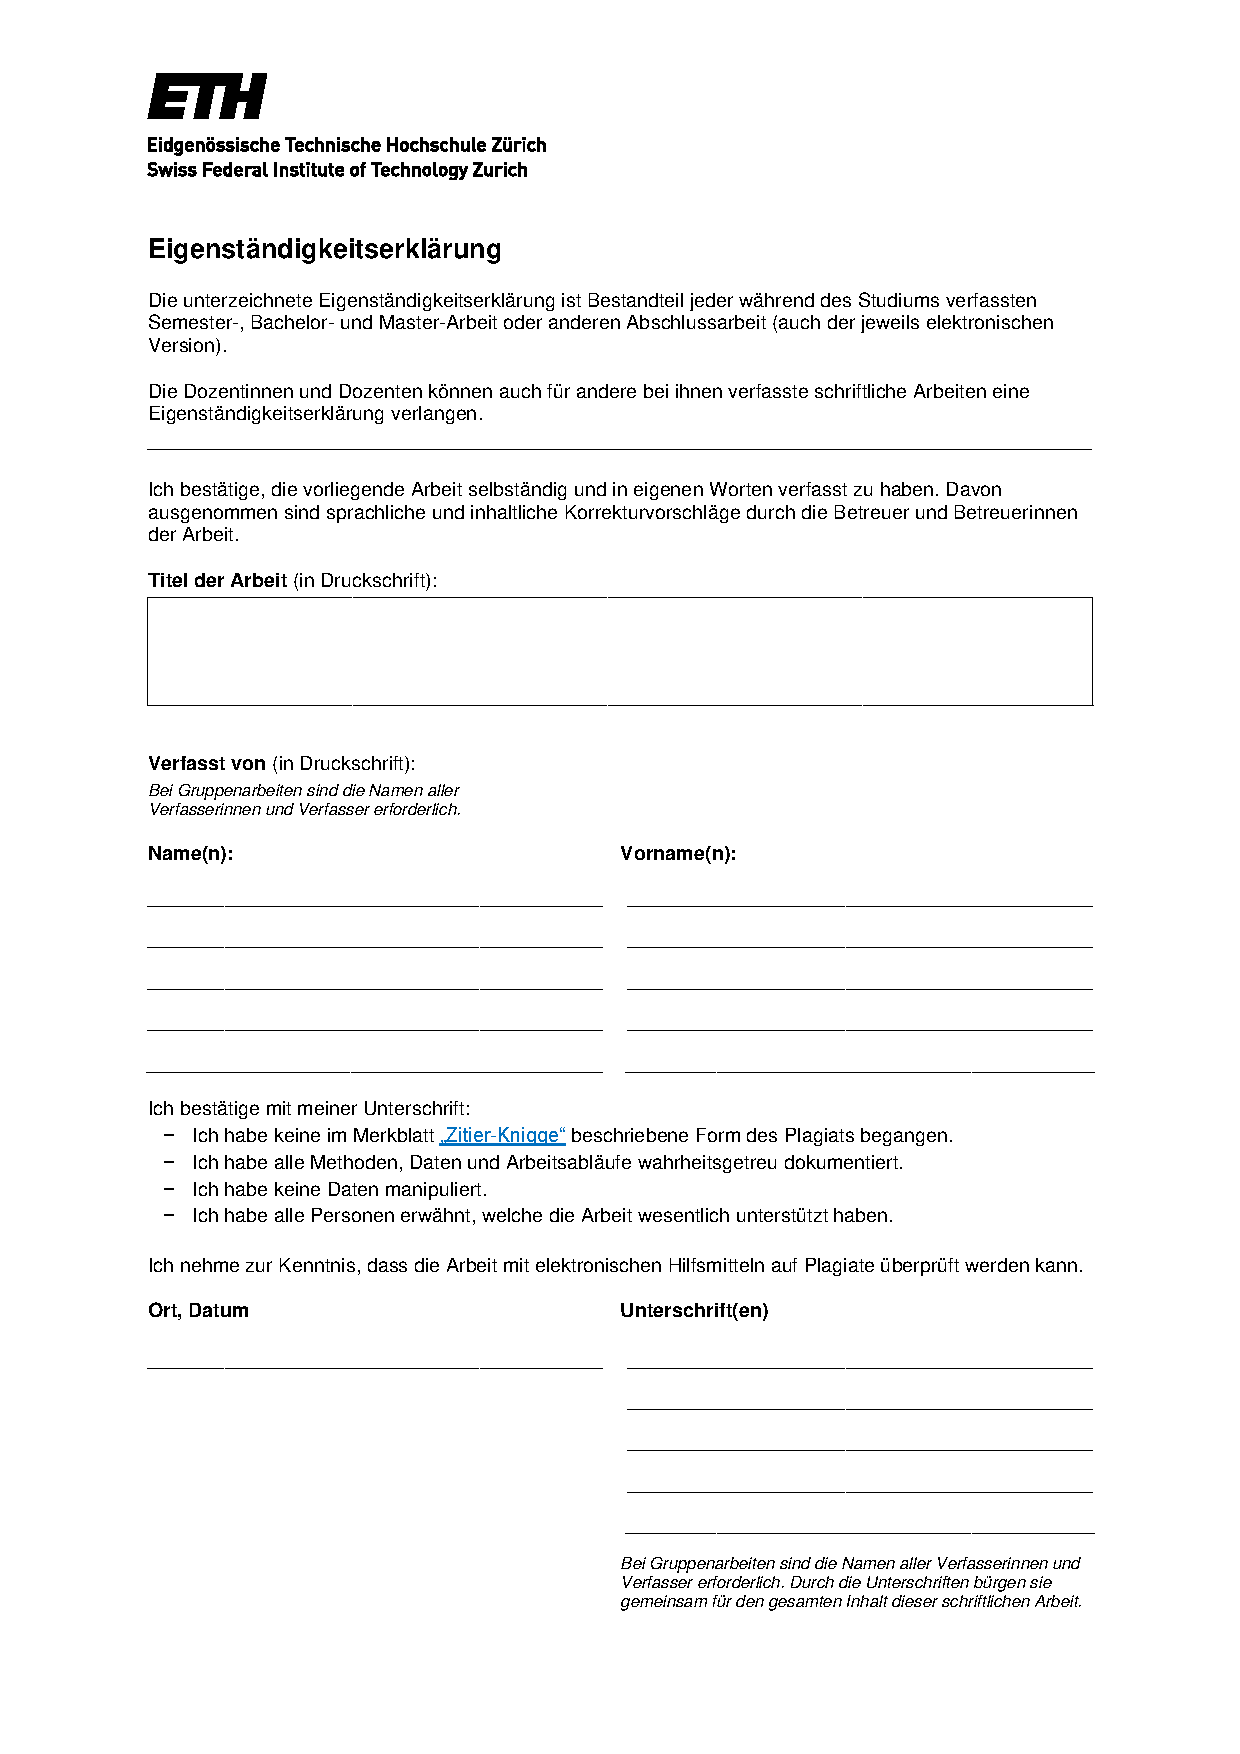
\includepdf[scale=0.8, pagecommand={}]{themen/pdfDateien/ethz_eigenstaendigkeitserklaerung.pdf}
\end{figure}



%%%%%%%%% --- Schlusswort --- %%%%%%%%%%

% Einfügen einer Leerseite ohne Seitenummer
\newpage
\thispagestyle{empty}
\mbox{}

% Schlusswort ohne Kapitelnummer mit Eintrag in ToC
\newpage
\addcontentsline{toc}{section}{Schlusswort}
\section*{Schlusswort}

Die hier vorliegenden \LaTeX-Rezepte sind entstanden aus Fragen die im Verlaufe der Zeit an mich gerichtet wurden. Fehlen für Sie interessante Themen und/oder Problemstellungen, senden Sie mir bitte eine Mail\footnote{peter.kessler@id.ethz.ch} und ich werde diese möglichst bald in dieses Dokument aufnehmen.

Haben Sie selber schon Lösungen/Beispiele zu Themen und/oder Problemstellungen die hier noch nicht enthalten sind, so können Sie mir diese sehr gerne zustellen, damit ich diese (natürlich mit Quellenangabe) in dieses Dokument aufnehmen kann.

\LaTeX\ ist nie Liebe auf den ersten Blick. \LaTeX\ lernt man (mit zunehmender Erfahrung/Übung) lieben. Je mehr \LaTeX-Rezepte hier versammelt sind, desto leichter fällt es zukünftigen Studierenden sich in \LaTeX\ einzuarbeiten.

Die hier gezeigten \LaTeX-Rezepte beschränken sich weitestgehend auf die Standards von \LaTeX. Vieles kann den eigenen Vorlieben angepasst werden. Um nur einige wenige Punkte aufzuzählen:

\begin{itemize}
\setlength\itemsep{-1em}
\item \textbf{Kapitelnummern:} Im \LaTeX-Standard hat die letzte Zahl einer Kapitelnummer keinen Punk. Hätte man gern auf hinter der letzten Zahl einer Kapitelnummer einen Punkt, kann dies entsprechend angepasst werden.  
\item \textbf{Titelseite:} Im \LaTeX-Standard hat die Titelseite lediglich drei Einträge (Titel, Autor und Datum). Im Standard können auch mehr als ein Autor angegbeen werden. Es ist auch möglich eine komplett selber gestalltete Titelseite zu erstellen. 
\item \textbf{Andere Packages:} Der \LaTeX-Standard deckt schon sehr viel ab. Zu verschiedenen Themen (Tabellen, Grafiken, Verzeichnisse, etv.) gibt es weitere Packages, mit viel mehr Einstellmöglichkeiten als im \LaTeX-Standard.  
\item \textbf{Verzeichnisse:} Die hier erstellten Verzeichnisse entsprechen dem Default-\LaTeX-Standard. Man kann auch hier alles gemäss eigenen Wünschen anpassen. Sollen die Verzeichnisse anders formatiert werden, sollen sie andere Titel haben, oder sollen in den Verzeichnissen kürzere Bezeichnungen (z.B. Tab. anstelle von Tabelle, Abb. anstelle von Abbildung, ...) verwendet werden - alles lässt sich mit mehr oder weniger Aufwand anpassen.
\item \textbf{...}
\end{itemize}

Beispiele zu oben geführten Themen sind im ausführlichen \LaTeX-Tutorial auf meinem GitHub-Repo\footnote{\url{https://github.com/pkmlp}}  zu finden. 

Dieses \LaTeX-Dokument wurde erstellt mit TeXmaker und getestet auf MacOS, Linux und Windows 10.

Nicht vergessen: \LaTeX\ ist nie Liebe auf den ersten Blick. \LaTeX\ lernt man erst (mit zunehmender Erfahrung/Übung) lieben. Darum erstellen Sie am besten alle Ihre Dokumente mit \LaTeX. Starten Sie nicht erst mit Ihrer Bachelor-/Master-Arbeit mit \LaTeX.


\end{document}
